%&latex
\documentclass[12pt]{okstate-thesis}
\usepackage{graphicx}
%\usepackage[draft]{graphicx}
%\usepackage{subfigure}
%\usepackage{verbatim}
%\usepackage{enumerate}
%\usepackage{amsmath}
%\usepackage{amscd}
%\usepackage{array}
%\usepackage{color}
%\usepackage{amsxtra}
%\usepackage{amstext}
%\usepackage{amssymb}
%\usepackage{hyperref}
%\usepackage{mathrsfs}
%\usepackage{latexsym}
%\usepackage{newlfont}
%\usepackage{indentfirst,color}
%\usepackage{doublespace}
%
\suppressfloats %\nofiles

\title{Phase Dithered Watermarking for Physical Layer Authentication}

\author{Nathan West}

\degreeone{Bachelor of Science in Electrical Engineering \\
        Oklahoma Christian University\\
        Edmond, OK\\
        2011}
\degreetwo{Bachelor of Nothing in Foo\\
        Prestigious University\\
        My head, Universe\\
        2012}
\degreesought{Master of Science}
\degreedate{May, 2013}
\majorfield{Electrical Engineering}
\adviser{George Scheets}
\chairOne{Keith Teague}
\chairTwo{Jim West}
%\chairThree{name 3}
%\chairFour{name}
% If you've got more you're screwed anyway, but you can read the class file
% to figure it out.
%
\begin{document}
\maketitle
\makeapproval{3} % Number denotes total number of required signatures (max 5)
\begin{acknowledge}
    I would like to thank....

\end{acknowledge}
\begin{abstract} % Creates abstract
    Abstract will go here.  Make sure it remains within the 350 word limit.

\end{abstract}
\tableofcontents
\listoftables
\listoffigures
%\msp    %========  single space text.
        %========  For the final version, this command should not be used.

%\makeapproval{5}\addtocounter{placeholder}{-1}    %% Comment this in the final copy. This is for electronic copy
%\begin{nomenclature}
%	\input{notation}
%\end{nomenclature}

%====================== main  body of the dissertation ==========================
\chapter{Oklahoma State University ECEN}
\section{A Letter from the Head}
Welcome to the School of Electrical and Computer Engineering (ECEN) at Oklahoma State University.

The School boasts 27 faculty members, including several IEEE Fellows and four recent and current NSF CAREER Award winners, along with approximately 300 undergraduate students and 150 graduate students pursuing the B.S., M.S. and Ph.D. degrees on both the Stillwater and Tulsa campuses. Students come to OSU from every state and approximately 120 countries making this a diverse, active, and exciting campus.

OSU offers a friendly and welcoming environment with easy access to faculty who are committed to excellence in the critical areas of teaching, scholarship and research. Our BS degree in Electrical Engineering is fully accredited by ABET. Your success as a student in ECEN is very important to us!

\begin{figure}
    \centering
    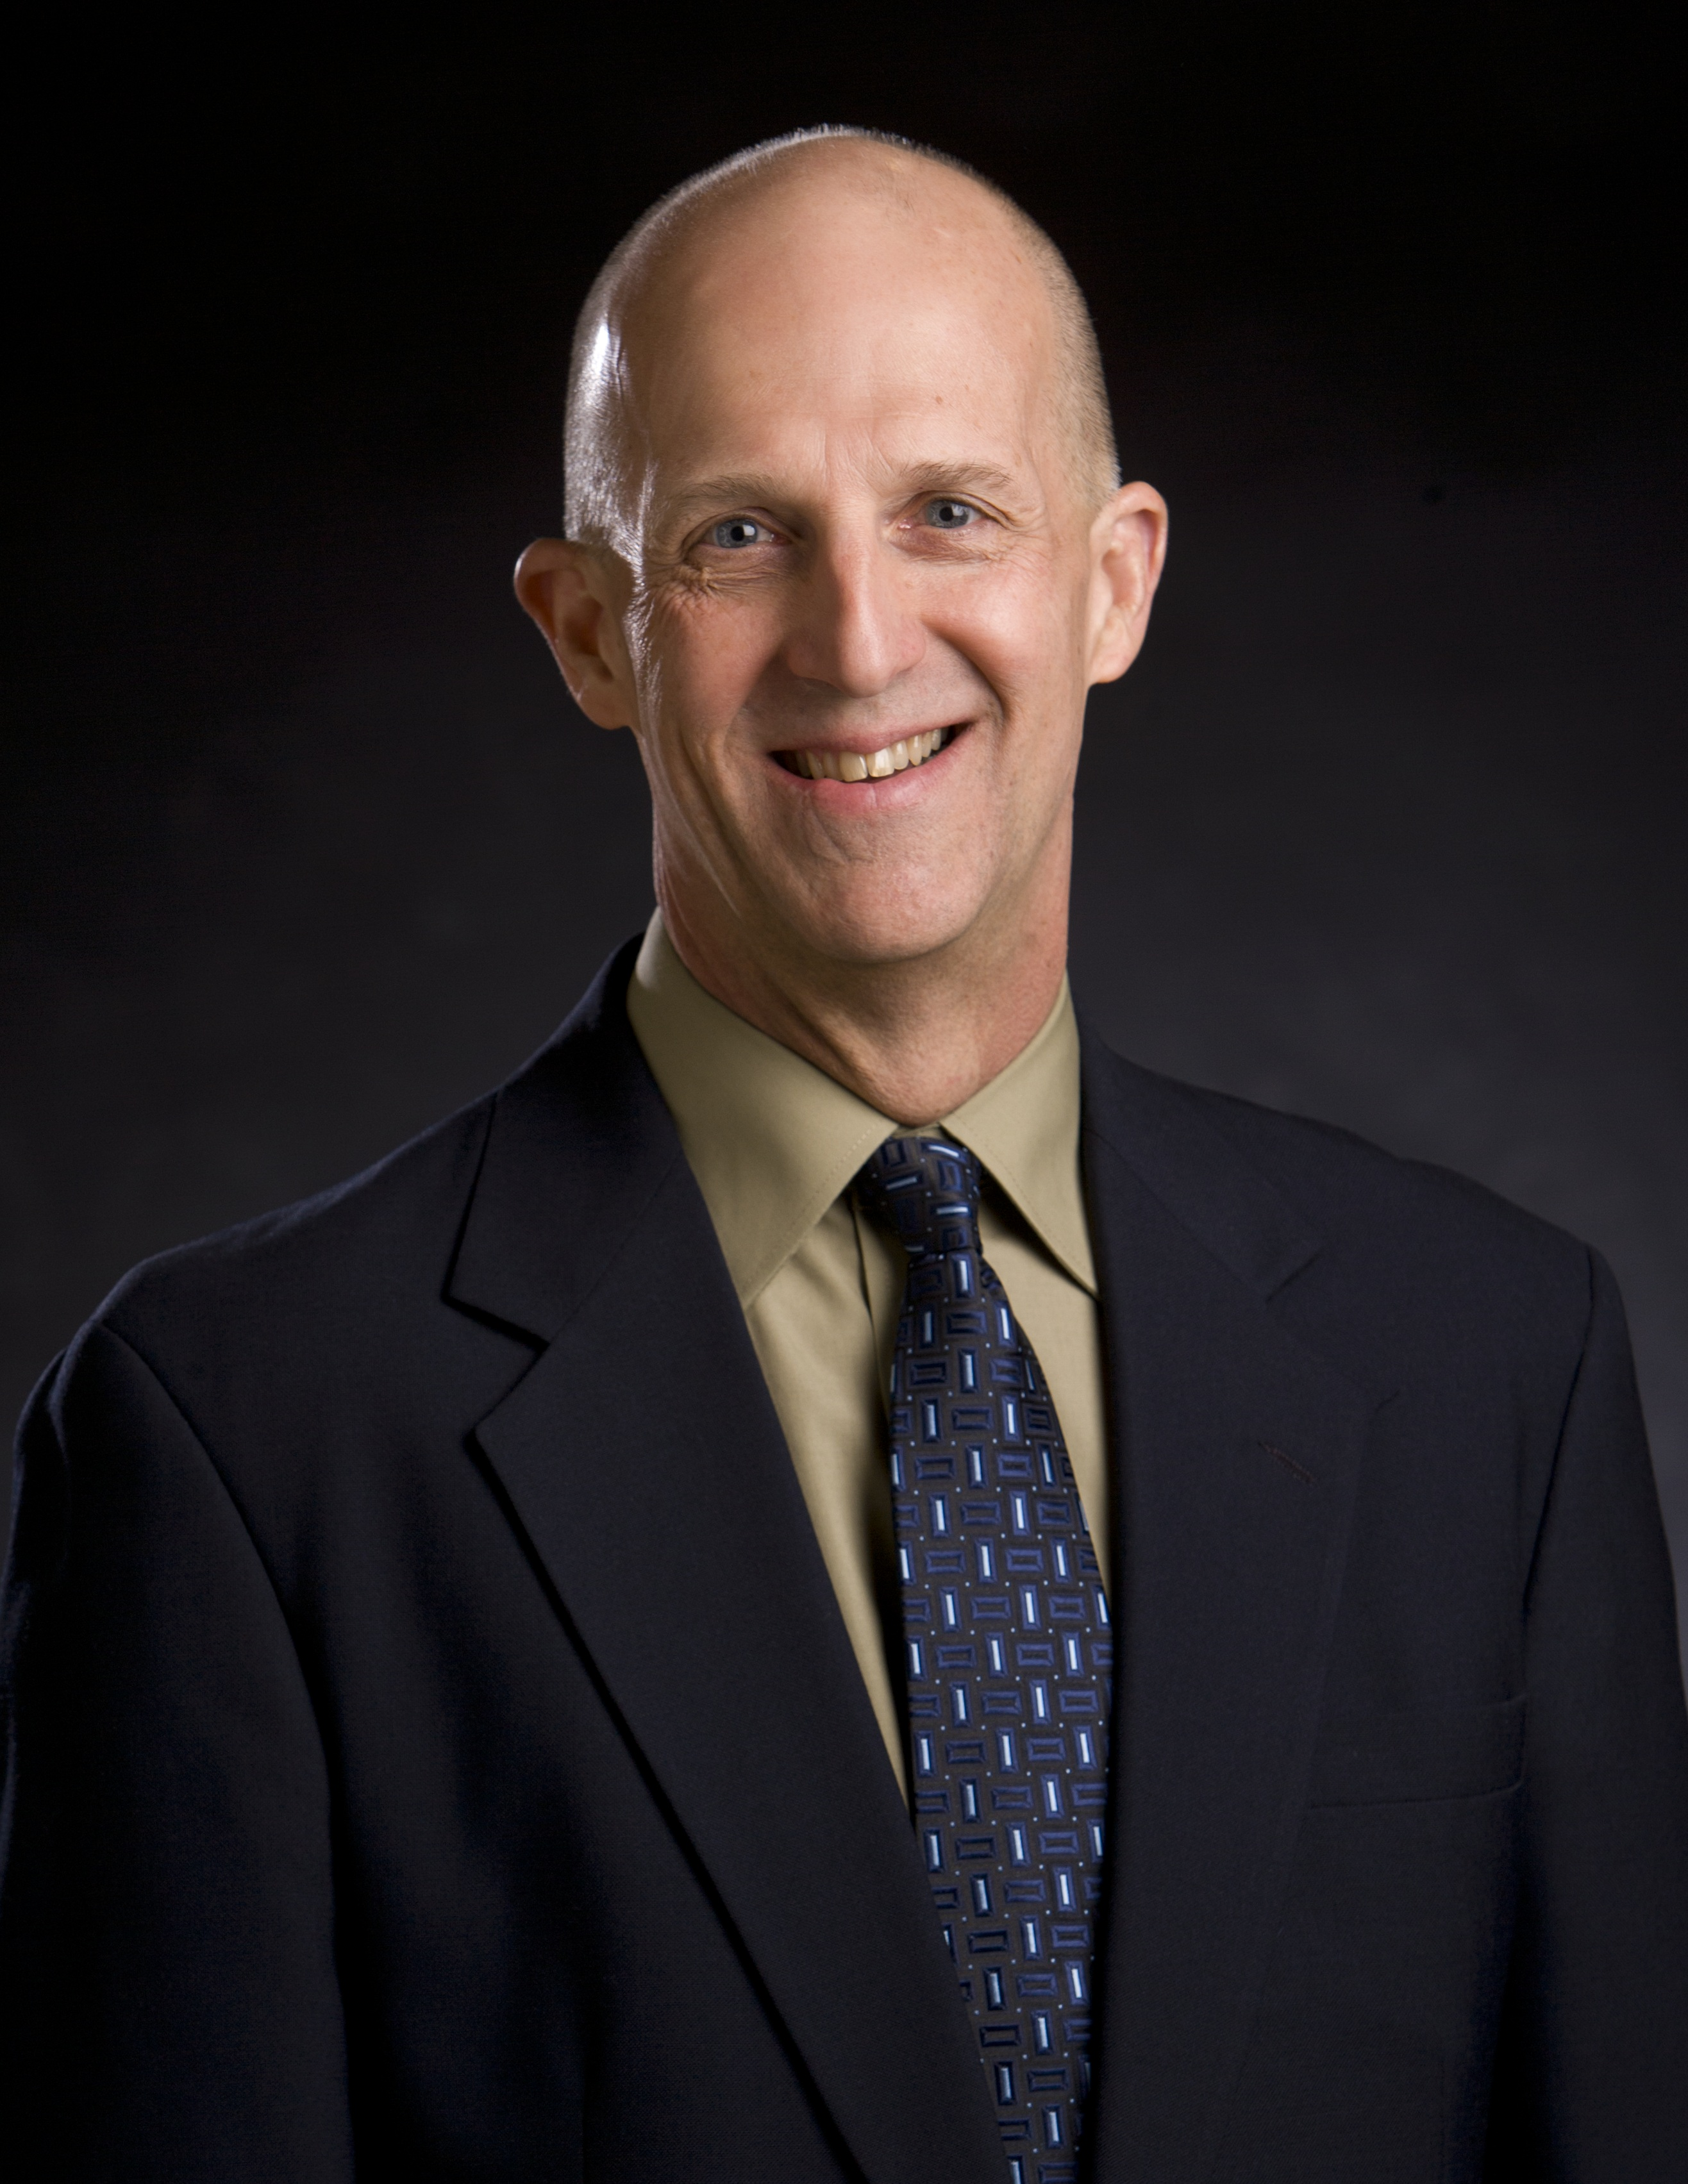
\includegraphics[width=0.25\columnwidth]{figs/DrTeague.jpg}
    \caption[Dr. Teague's Head]{Dr. Teague, Professor, Department Head}
\end{figure}
    

Over the past three years the School has experienced an unprecedented period of growth. We have been very fortunate to welcome nine new faculty members in the areas of computer engineering, communications, image processing and machine vision, biomedical engineering, and nanotechnology. We strive to emphasize excellence in all area of instruction, scholarship and research, as evidenced by a growing list of faculty and student accomplishments. Research and scholarly activities continue to expand, and thanks to an outstanding faculty annual research funding totals over $\$3.5$ million.

Our programs center around five primary thrust areas: communications, controls, and signal processing; computer engineering; lasers and photonics; electronics and mixed signal VLSI; and power. There are opportunities within these areas to accommodate the goals of almost any student interested in the various specializations within Electrical Engineering and Computer Engineering, as well as several interdisciplinary areas. We are especially excited about a new BS degree in Computer Engineering that we expect to introduce in 2008.

Excellent instruction and research laboratories are located in Engineering South and the Advanced Technology Research Center, a world-class facility located adjacent to Engineering South on the Stillwater campus. In Tulsa, the new Helmerich Advanced Technology Research Center houses a growing program in advanced materials and nanotechnology. 

Engineering graduates are in very high demand with over 170 companies actively recruiting at the most recent engineering career fair on campus. Our graduates are recognized as great employees who command high salaries. Our graduates are equally well prepared to study for an advanced degree, and many choose to pursue the M.S. or Ph.D. degree either at OSU or another outstanding university.

I’m very excited about our programs and what we have to offer. Please feel free to contact any faculty member or me for further information.

\subsection{ECE Mission Statement}

The School of Electrical and Computer Engineering – serving the needs of students, faculty, and those who employ our graduates – provides a comprehensive education in electrical or computer engineering. By providing both a breadth of knowledge and depth with design experience in selected areas, graduates are prepared to continue the lifelong process of education needed by active professionals in today's constantly changing global society.


\chapter{ECEN Graduate Program}

Degree programs are offered at the M.S. and Ph.D. levels in Electrical Engineering. Major areas of emphasis in both course offerings and research include communications, speech and image processing, laser applications, computer systems, digital and analog VLSI design, electronics, control theory, real-time system control, renewable energy systems, electric power economics, microwave remote sensing, expert system development, and parallel processing. More details about state-of-the-art research laboratories can be found here.

For more information, contact the School, or Dr. Ramakumar, the ECEN Graduate Coordinator.


\section{MS Degree Program}
Two Master's degree options are available to students in Electrical and Computer Engineering.

\begin{itemize}
\item MSEE (Traditional Thesis Path)  Plan I:*    30 Hours
\item MSEE (Professional Path)    Plan III:*  33 Hours
\end{itemize}

*Plan I, Plan III, etc., refers to Graduate College designation.
Students in the Professional Path (Plan III) are required to take courses in at least four areas of ECEN at the 5000 level (designated by second digit of course number). Students in the Traditional Thesis Path (Plan I) are required to take courses in at least two areas of ECEN at the 5000 level (designated by the second digit of course number). A summary of the two degree program requirements is given in the following table:

\begin{table}
    \centering
    \caption[ECEN MS Requirements]{The credit requirements for an MS in ECEN at OSU. Depending on desired path different classes are required in different areas. In the end you get to pick whatever you want!}
    \begin{tabular}{l c c}
        & Traditional Path & Professional Path \\
        \hline \hline
        Technical Elective          & 3 hours   & 3 hours  \\
        ECEN Graduate Level Courses & 18 hours  & 21 hours \\
        Additional Courses          &           & 6 hours  \\
        Thesis                      & 6 hours   &          \\
        ECEN 5070                   & 3 hours   &          \\
        Creative Component          &           & 3 hours  \\
        \hline
                                    & 30 hours  & 33 hours \\
    \end{tabular}
\end{table}

For Professional Path option (Plan III), a 3-hour ECEN 5000+ course (with a term project) is designated as the creative component. Or, a 3 hour ECEN 5070 may be completed, under the supervision of an ECEN professor. For the Traditional Path option (Plan I), the optional 3 hours of ECEN 5070 should be completed with the thesis advisor.

Additional Master's degree requirements are:

\begin{enumerate}
    \item Professional Path students MUST take 6 hours from ECEN 5513, 5613, 5713 and any remedial courses at the first enrollment opportunity after entrance into the MS program.
    \item Traditional Path students MUST take 3 hours from ECEN 5513, 5613 and any remedial courses at the first enrollment opportunity after entrance into the MS program.
    \item Up to two (2) 4000 level ECEN courses that have been approved for graduate credit within the ECEN program may be included on the Master's plan of study. The list of approved courses is included at the end of this bulletin.
    \item No course required for the BSEE degree at OSU may appear on a study plan for the Master's degree.
    \item No course that was applied to BSEE credit may be included on a graduate plan of study.
    \item The minimum requirement of 18 hours of graduate-level courses in ECEN MAY NOT include the following courses: ECEN 5000, 5030 and 6050.
    \item CS 4113 IS NOT appropriate for M.S. Plans of Study in this department.
    \item Graduate College regulations REQUIRE a minimum of 21 hours of 5000-level courses on all Master's plans.
    \item Students who do not have a BSEE degree CAN include only one "outside" course on their Master's Plan of Study. All students MUST have at least one course "outside" ECEN.
    \item For the technical elective (3 hours), courses that are cross-listed with ECEN must be approved by the student's advisor.
\end{enumerate}

\subsection{Entrance Requirements}

3.0 GPA in an accredited BSEE program is the usual standard for admission to the MSEE program. However, applicants with lower GPA, to about 2.7, may be granted probationary admission. Students who have BS degrees in other engineering fields may be admitted to the MSEE program, subject to the same GPA requirements. These candidates will be expected to take enough prerequisite courses (from undergraduate ECEN courses, and perhaps some Math, CS and Physics) to accomplish two ends: (a) to assure a reasonable basis for success in the graduate courses to be taken for the MSEE degree; and, (b) to assure that when the candidate goes into practice with the MSEE degree, there will be no potentially "embarrassing holes" in the candidate's technical background. This may well require some prerequisite courses in areas of study in which the student has little interest and in which he/she has no intention of practicing after graduation. Students are sometimes admitted to an MSEE program with a grade of "C" in one or two junior or senior courses. Students may be required, as a condition of admission to the MSEE program; to repeat such courses, or take another undergraduate -level course in the same or closely-related area of study. A grade of "B" MUST be attained in such prescribed prerequisites.
Students admitted unconditionally to the program are assumed competent to take the required M.S. courses. If the student feels unprepared for one of the required classes, he/she may enroll in the appropriate prerequisites.
Students admitted conditionally should enroll in the necessary undergraduate prerequisites as a first priority. Graduate courses may be taken concurrently with prerequisite courses in other areas. The student need not necessarily complete all prerequisite courses before taking the first 5000-level courses.
GRADUATE RECORD EXAMINATION: Scores for the Graduate Record Examination (GRE) general exam must be submitted with the application.

\subsection{Retention Standards}

The Graduate College bulletin sets forth certain minimum grade standards for retention: The School of Electrical and Computer Engineering expects all candidates to attain grades of "B" in all courses taken as graduate students, whether prerequisite courses or courses listed as part of the Plan of Study. A grade below "B" in a prerequisite course is cause for suspension. A 3.0 or above GPA in graduate courses must be maintained. A grade below "C", or more than two (2) "C's" in graduate courses will result in suspension.

\subsection{Master of Science Degree}

Graduate College credit requirements for the Master of Science degree may be satisfied by one of the following alternatives:

A thesis of NOT MORE than 9 credit hours, plus 21 (or more) hours of course work for a total of 30 hours. (Graduate College Plan I)
33 hours of approved course work which MUST include a three-hour creative component (course or independent study). (Graduate college Plan III ).
Note that Graduate College Plan II, the report option IS NOT available to ECEN students.

A preliminary Plan of Study for the Master's Degree should be worked out by the student and his/her advisor. This plan should include a listing of course work contemplated, and an estimate of the time schedule. All Master of Science degree students must satisfy the creative component requirement of the Graduate College. For students electing the Plan III option, at least 3 hours must be designated with the advisor's approval, as the creative component (which may include independent study ). The initiative for proposing a plan of study lies with the student; the student should note the Graduate College requirement that a Master's plan be filed BEFORE the student registers for his/her 17th hour of graduate credit. A creative component proposal MUST ALSO BE approved and filed.

The approval of the student's advisor and two other faculty members as well as that of the Dean of the Graduate College is required on all Master's Plans of Study. The student should work out his proposed plan of study with his advisor and arrange for typing and submission of the final version to the graduate college.

Study plans may be revised from time to time; the revision is accomplished by submitting a new plan as outlined above. The Graduate College REQUIRES that the final plan be filed before registration for the semester in which the necessary work for the degree will be completed.

The School of Electrical and Computer Engineering waives the foreign-language requirement for Master's Degree.

\section{PhD Degree Program}
The PhD Degree has different requirements. When they become relevant to me next year I'll look at them!

\section{Other Graduate Degree Options}
There's apparently some other degrees. I don't care really care about them.

\section{Department Forms}
There are a variety of forms.
\begin{itemize}
    \item Graduate Memorandum
    \item Plans of Study Forms
    \item Masters
    \item Ph.D.
    \item Graduation Clearance Form
    \item Assistantship
    \item Assistantship Applications
    \item International Teaching Assistant Program
\end{itemize}

%
\nocite{*} % Use to exclude specific citations from *.bib file
\bibliography{communications}
\bibliographystyle{ieeetr}%{alpha}%{ieeetr}%%
\appendix
\chapter{IMPORTANT TABLE}\label{chap:appA}
 Appendix~\ref{chap:appA} goes here.  Table~\ref{tbl:appA:table1} is copied from Chapter~\ref{chap:chap3}.
 %
\begin{table}[h]
\caption{Sample multicolumn table}
\begin{center}
  \begin{tabular}{|l|cc|cc|}
    \hline
  Parameter & \multicolumn{2}{c|}{Column 1} & \multicolumn{2}{c|}{Column 2}\\ \cline{2-5}
              & Subcolumn 1 & Subcolumn 2 & Subcolumn 1 & Subcolumn 2 \\
\hline
    Parameter 1 & Element 11 & Element 12 & Element 13 & Element 14\\
    Parameter 2 & Element 21 & Element 22 & Element 23 & Element 24\\
    Parameter 3 & Element 31 & Element 32 & Element 33 & Element 34\\
    \hline
\end{tabular} \label{tbl:appA:table1}
\end{center}
\end{table}
%
\chapter{MORE DATA}\label{chap:appB}
Appendix~\ref{chap:appB} data goes here

\newpage
 \begin{vita}{Your Name}{Doctor of Philosophy}{Your Major} %Creates vita
 \vitaitem{Personal Data:} Born in City, State, Country on Month Day, YEAR.             
 \vitaitem{Education:} \\ Received the B.S. degree from ???, City, State, Country, YEAR, in Major \\
Completed the requirements for the degree of Master of Arts/Science with a major in your major Oklahoma State University in Month, YEAR.
\vitaitem{Experience:} \\ Any work experience attained
  \end{vita}

%       \pagestyle{empty}

\end{document}
